\section{Multigrid Methods}\label{sec:multigrid-methods}
%Multigrid methods aim to accelerate the convergence of iterative methods by eliminating certain error components more efficiently on a coarser resolution of the same problem.
While basic iterative methods, such as Jacobi and Gauss-Seidel, are applicable to many PDE-based problems, in practice, their speed of convergence is often insufficient, which means that a large number of iterations is required until an acceptable approximation accuracy can be attained. 
The main reason for this behavior is that these methods are only efficient in the reduction of certain error components, while others remain mostly unaffected~\cite{briggs2000multigrid}.
This can be best understood by investigating their effect on oscillatory errors with different frequencies.
For this purpose, we consider the one-dimensional Laplace equation
\begin{equation}
		\begin{split}
			- \Delta u(x) & = 0 \quad \forall x \in (0, 1) \\
			u(0) & = u(1) = 0,
		\end{split}
		\label{eq:1D-laplace-model}
\end{equation}
which is discretized using the three-point stencil
\begin{equation}
	- \Delta_h = \frac{1}{h^2}\begin{bmatrix}
		-1 & 2 & -1
	\end{bmatrix}.
		\label{eq:1D-laplace-stencil}
\end{equation} 
Figure~\ref{fig:different-error-components} shows the impact of applying the Jacobi and Gauss-Seidel method to different periodic error components.
\begin{figure}
	\centering
	\begin{subfigure}[t]{0.32\textwidth}
		\centering
		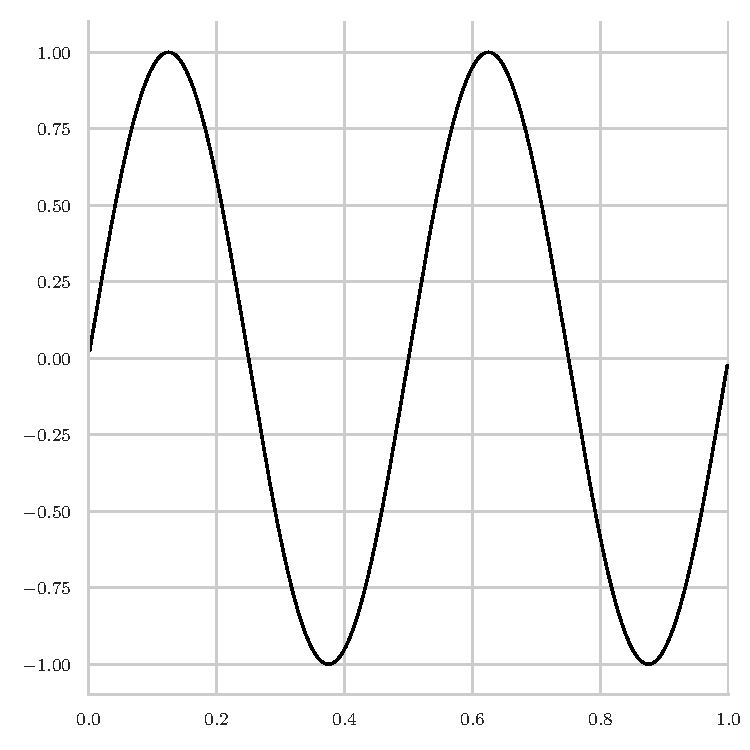
\includegraphics[width=\textwidth]{figures/error_plots//initial_error_jacobi_4pi.pdf}
		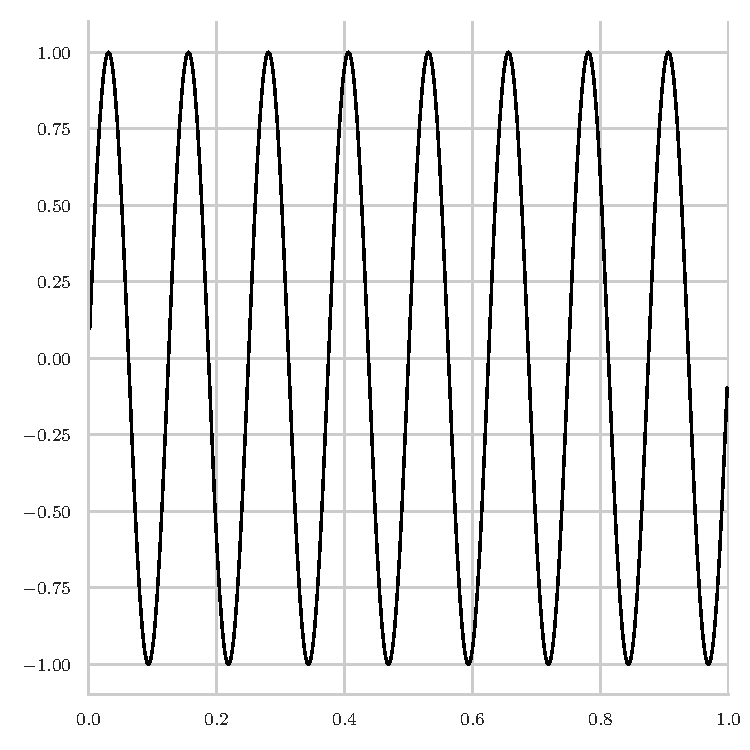
\includegraphics[width=\textwidth]{figures/error_plots//initial_error_jacobi_16pi.pdf}
		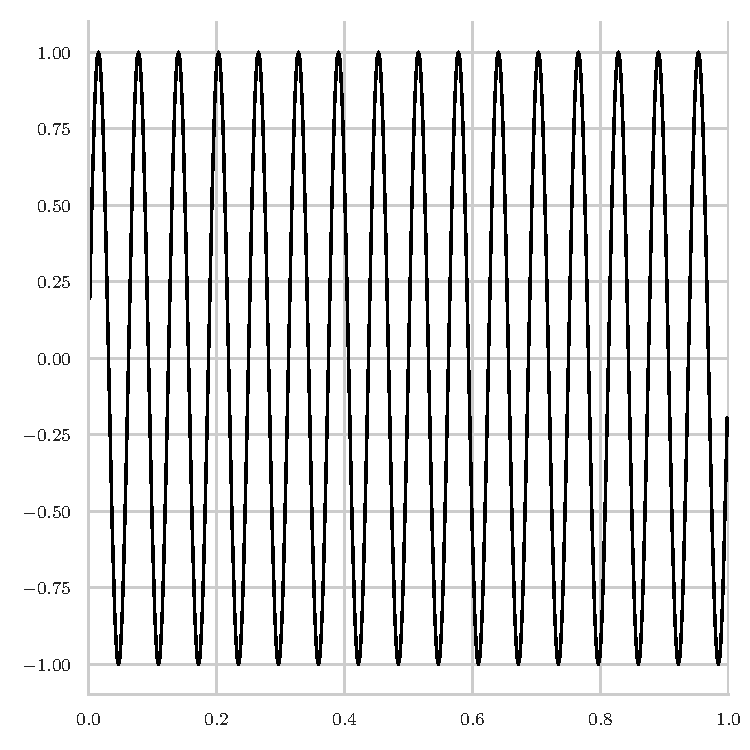
\includegraphics[width=\textwidth]{figures/error_plots//initial_error_jacobi_32pi.pdf}
		\caption{Initial error}
	\end{subfigure}
	\hfill
	\begin{subfigure}[t]{0.32\textwidth}
		\centering
		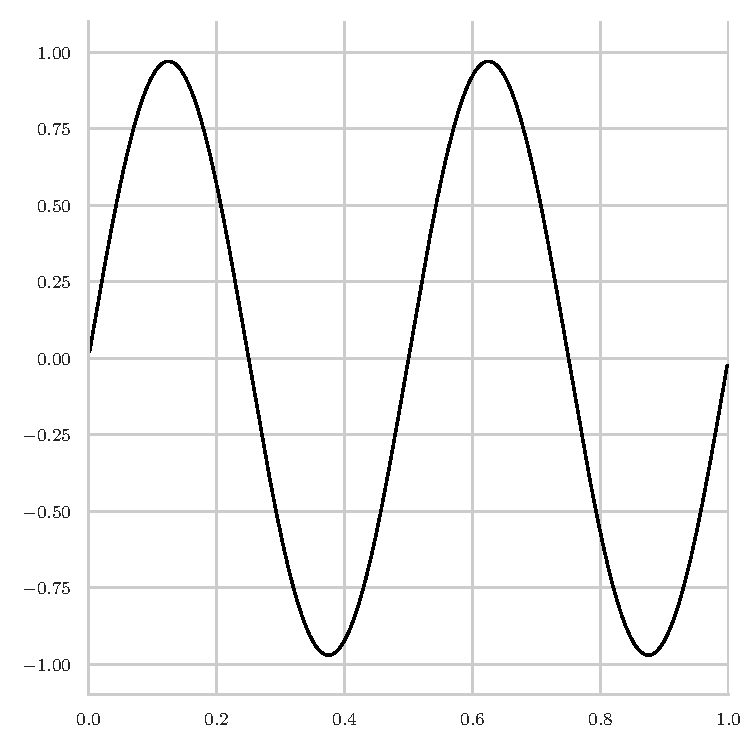
\includegraphics[width=\textwidth]{figures/error_plots//final_error_jacobi_4pi.pdf}
		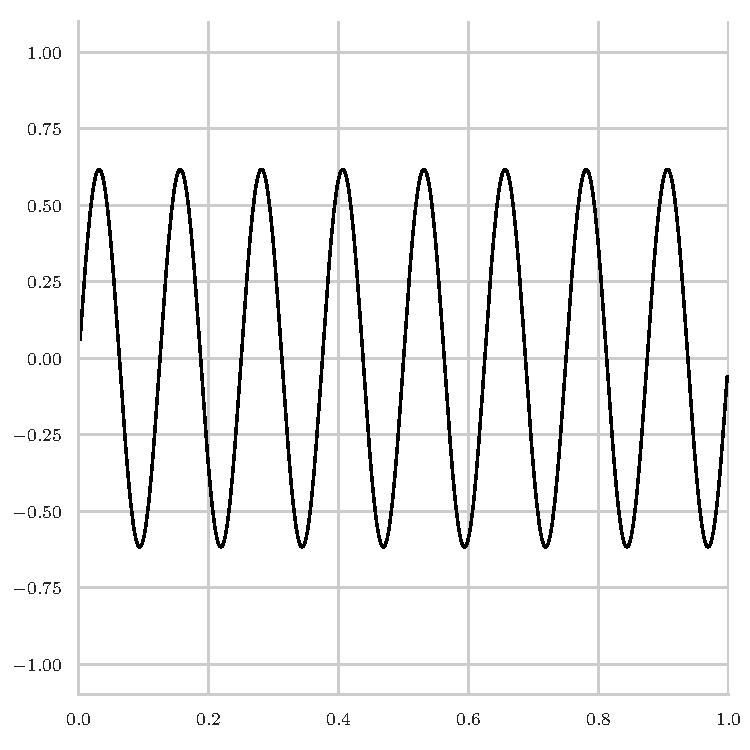
\includegraphics[width=\textwidth]{figures/error_plots//final_error_jacobi_16pi.pdf}
		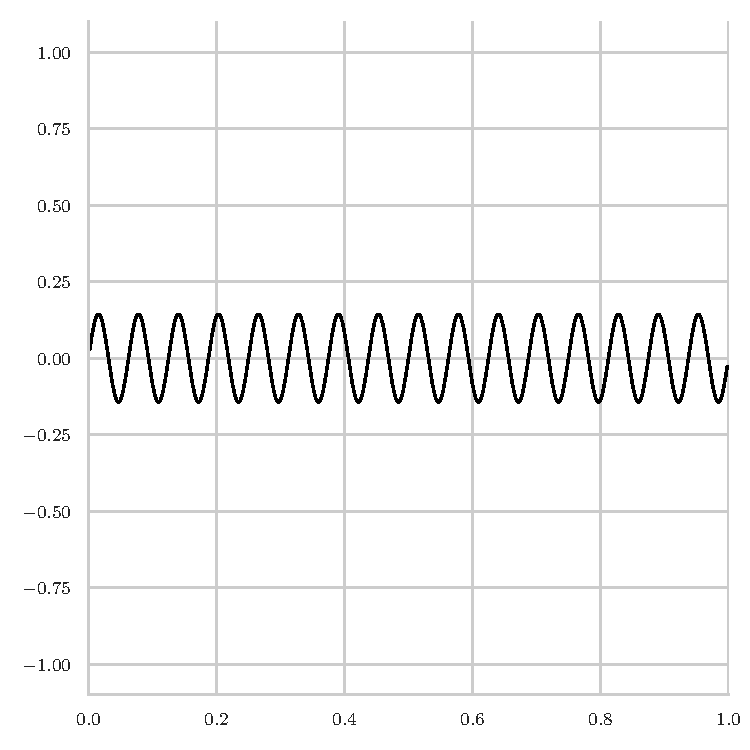
\includegraphics[width=\textwidth]{figures/error_plots//final_error_jacobi_32pi.pdf}
	\caption{Error after applying Jacobi}
	\end{subfigure}
	\hfill
	\begin{subfigure}[t]{0.32\textwidth}
		\centering
		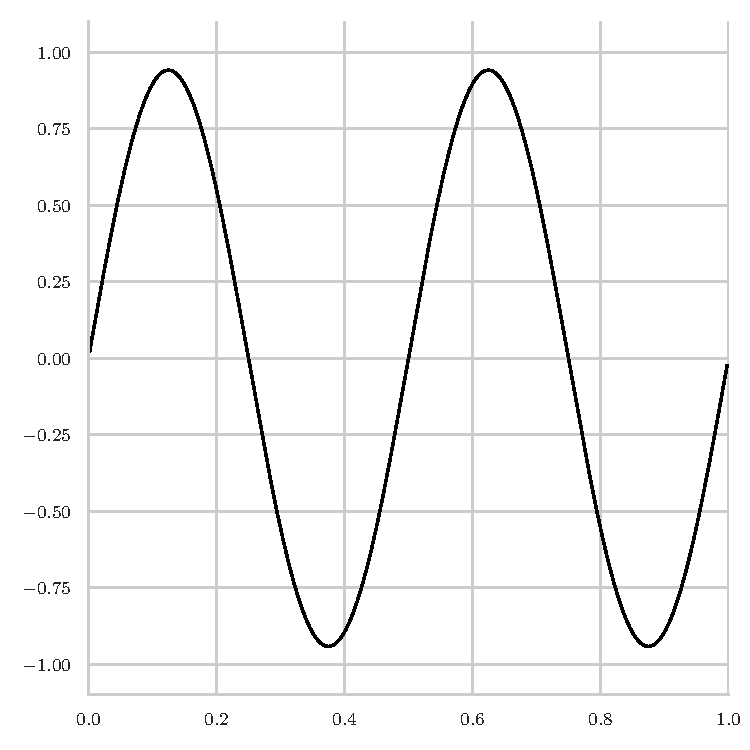
\includegraphics[width=\textwidth]{figures/error_plots//final_error_gauss_seidel_4pi.pdf}
		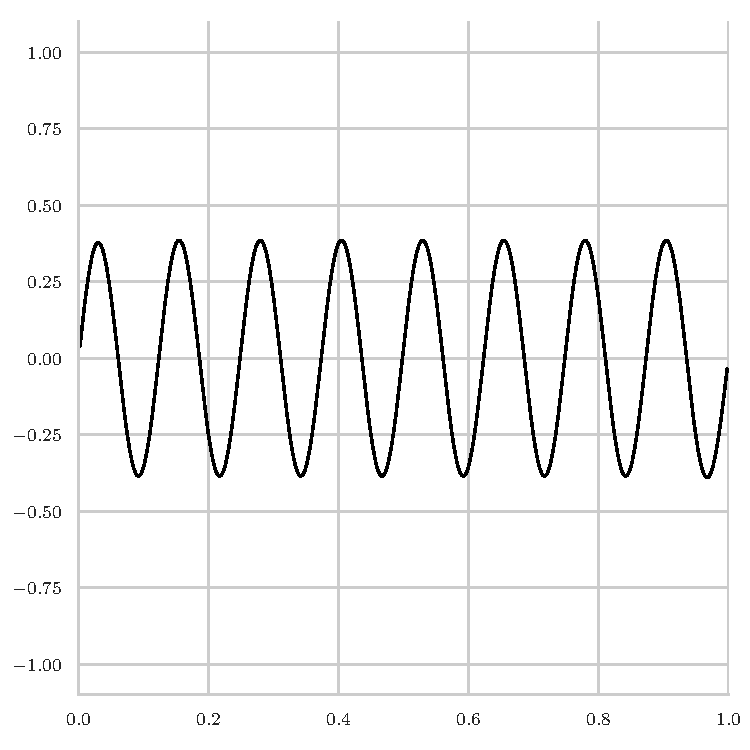
\includegraphics[width=\textwidth]{figures/error_plots//final_error_gauss_seidel_16pi.pdf}
		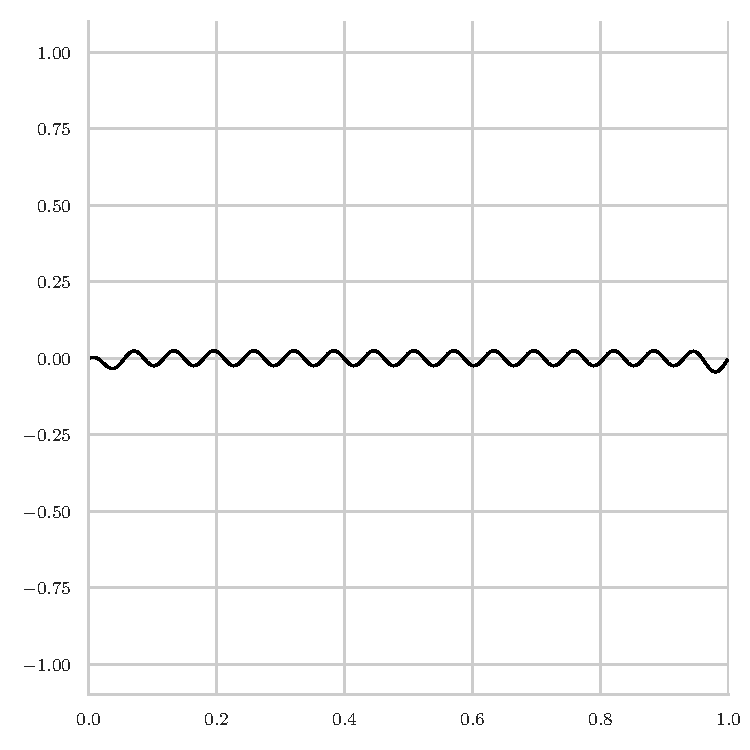
\includegraphics[width=\textwidth]{figures/error_plots//final_error_gauss_seidel_32pi.pdf}
	\caption{Error after applying GS}
	\end{subfigure}
	\caption{Different error components on a one-dimensional grid with step size $h = 2^{-9}$ before and after applying 100 steps of the Jacobi or Gauss-Seidel (GS) method.}
	\label{fig:different-error-components}
\end{figure}
Here, the first column shows the initial error discretized on a grid with step size $h = 2^{-9}$ while the second and third include the remaining error after applying 100 Jacobi and Gauss-Seidel steps, respectively.
Note that the frequency of change increases from top to bottom, whereas the amplitude of the error is always the same.
As can be seen in the second and third column of the first row of Figure~\ref{fig:different-error-components}, the Jacobi and Gauss-Seidel methods do not yield a significant reduction of the low-frequency error components within 100 iterations.
In contrast, in the third row, which shows a highly-oscillating component, the application of 100 steps of the Jacobi method already reduces the initial error to less than one-fifth of its original value.
The same behavior can also be observed for the Gauss-Seidel method, whereby, compared to the Jacobi method, high-frequency error components are reduced even faster.
We can further illustrate the error reduction properties of basic iterative methods by investigating Figure~\ref{fig:combined-error}, which contains a combination of two error components with equal magnitude, one of them with low and the other one with high frequency.
\begin{figure}
	\begin{subfigure}[t]{0.32\textwidth}
	\centering
		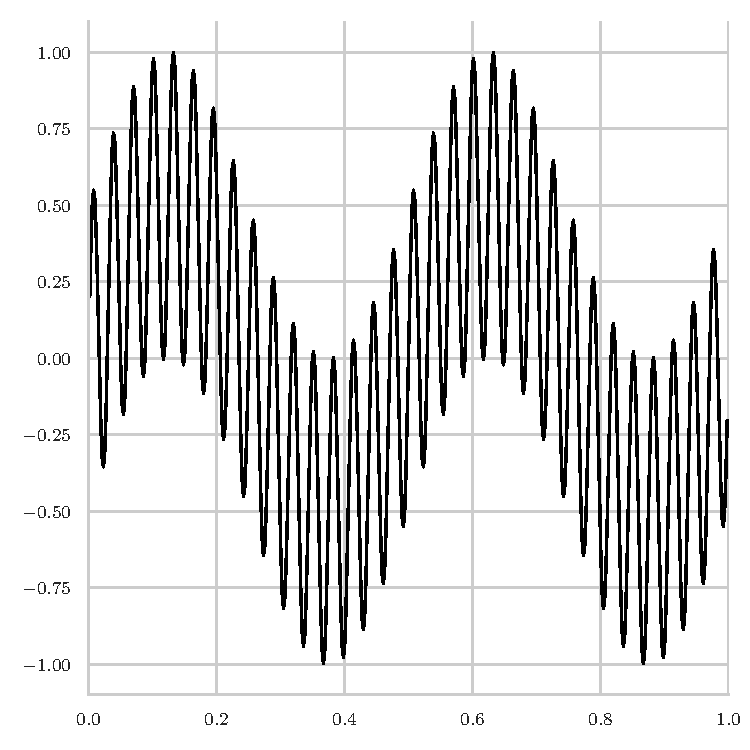
\includegraphics[width=\textwidth]{figures/error_plots//initial_error_jacobi_combined.pdf}
		\caption{Initial error}
\end{subfigure}
\hfill
\begin{subfigure}[t]{0.32\textwidth}
	\centering
		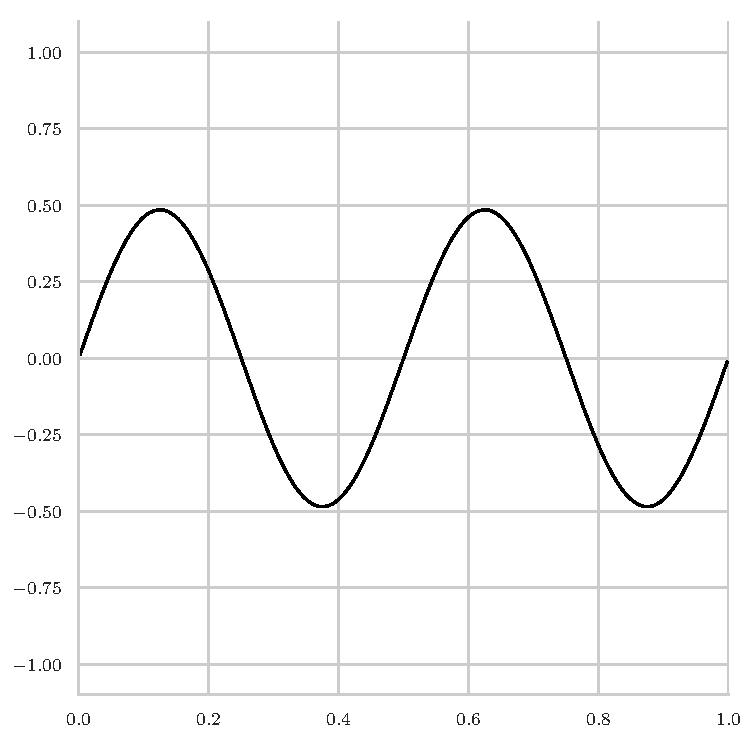
\includegraphics[width=\textwidth]{figures/error_plots//final_error_jacobi_combined.pdf}
		\caption{Error after applying Jacobi}
\end{subfigure}
\begin{subfigure}[t]{0.32\textwidth}
	\centering
	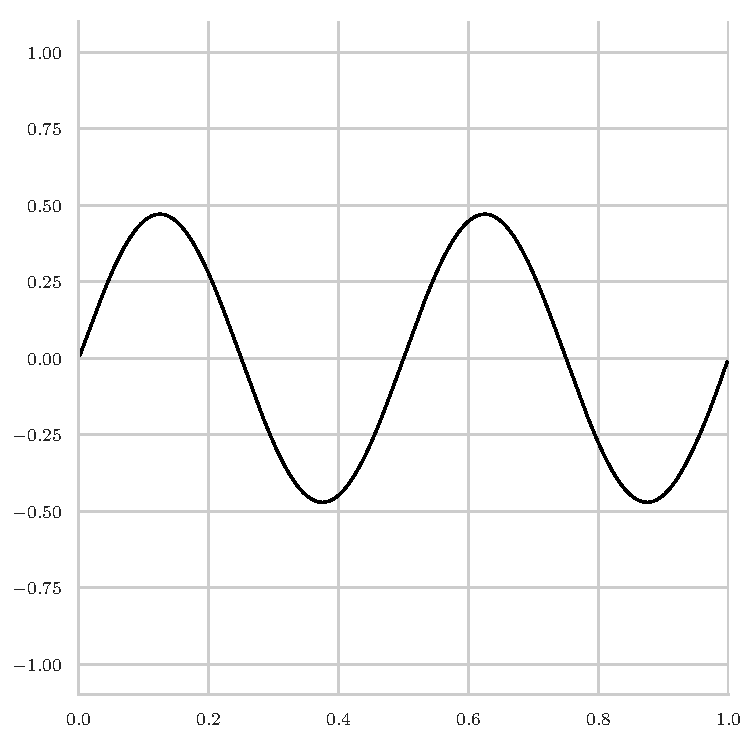
\includegraphics[width=\textwidth]{figures/error_plots//final_error_gauss_seidel_combined.pdf}
	\caption{Error after applying GS}
\end{subfigure}
	\caption{Combination of two error components discretized on a one-dimensional grid with step size $h = 2^{-9}$ before and after applying 100 steps of the Jacobi or Gauss-Seidel (GS) method.}
\label{fig:combined-error}
\end{figure}
Again, the first plot shows the initial error, while the second and third contain the reduced error after 100 iterations of Jacobi and Gauss-Seidel, respectively.
In accordance with our previous observations, the attained improvement achieved with both methods can be almost fully attributed to the reduction of the highly-oscillating component.
Because the remaining error is more smooth than initially, basic iterative methods are often called \emph{smoothers}, and their effectiveness is measured in terms of their capability to reduce the high-frequency components of a given error. 

Now observe what happens if we represent the same low-frequency error component shown in the first row of Figure~\ref{fig:different-error-components} on a grid with larger step size $h = 2^{-6}$ and, thus, a smaller number of grid points.
Because the number of (inner) grid points $n = 1/h - 1$ is inversely proportional to the step size, we call such a grid \emph{coarser}.
The resulting error reduction, again after 100 iterations of each method, is shown in Figure~\ref{fig:low-frequency-error-component-coarse}. 
\begin{figure}
	\begin{subfigure}[t]{0.32\textwidth}
	\centering
	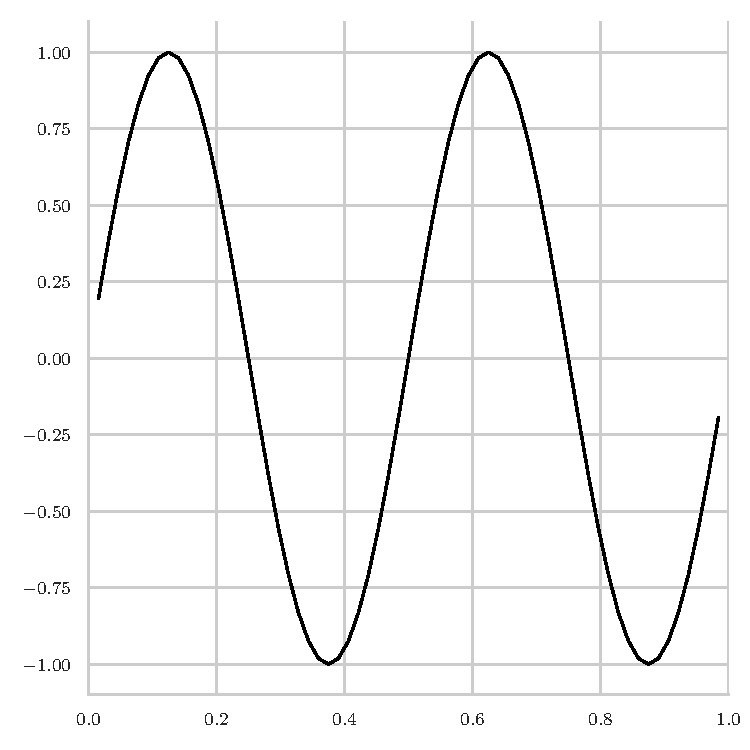
\includegraphics[width=\textwidth]{figures/error_plots//initial_error_jacobi_4pi_coarse.pdf}
	\caption{Initial error}
\end{subfigure}
\hfill
\begin{subfigure}[t]{0.32\textwidth}
	\centering
	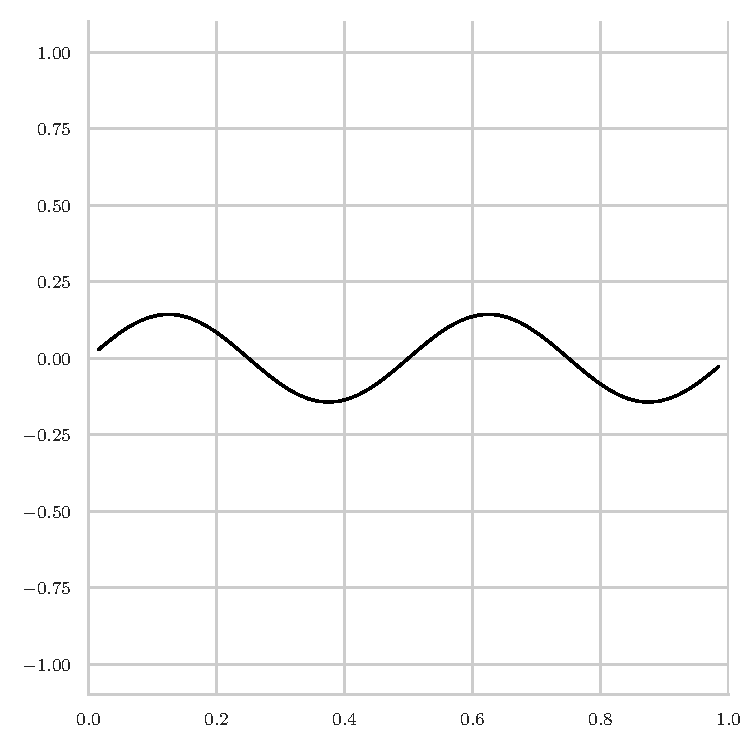
\includegraphics[width=\textwidth]{figures/error_plots//final_error_jacobi_4pi_coarse.pdf}
	\caption{Error after applying Jacobi}
\end{subfigure}
	\hfill
	\begin{subfigure}[t]{0.32\textwidth}
		\centering
		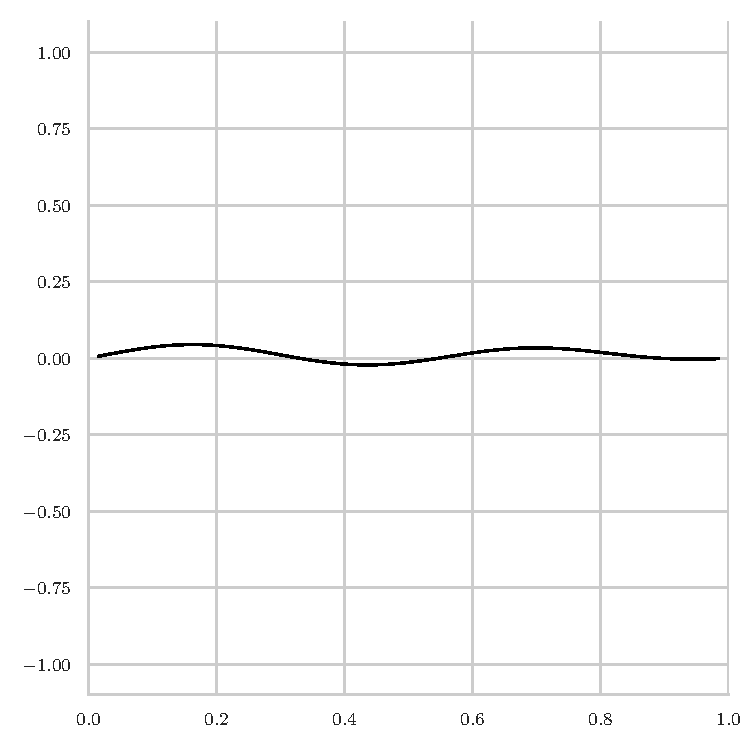
\includegraphics[width=\textwidth]{figures/error_plots//final_error_gauss_seidel_4pi_coarse.pdf}
		\caption{Error after applying GS}
	\end{subfigure}
	\caption{Low-frequency error component discretized on a coarser one-dimensional grid with step size $h = 2^{-6}$ before and after applying 100 steps of the Jacobi or Gauss-Seidel (GS) method.}
	\label{fig:low-frequency-error-component-coarse}
\end{figure}
As it can be seen, the amount of low-frequency error reduction is significantly higher for both methods than on the \emph{finer} grid with a step size of $h = 2^{-9}$.
While smoothers, such as Jacobi and Gauss-Seidel, are only effective in reducing the high-frequency components of a given error, we can overcome this limitation by representing the remaining error on a coarser grid.
Since, on this level, the remaining low-frequency components become more oscillatory, smoothing regains its effectiveness. 
\emph{Multigrid} methods extend this idea by recursively obtaining a coarser representation of the same problem, whose error can then be effectively reduced by employing only a few \emph{smoothing} iterations.
The result is then used to extinguish the remaining error on the next-higher level.
In the following, we introduce the basic components of multigrid methods, i.e., the smoothing, restriction, prolongation, and coarse-grid correction operations.
%Based on this definition, we then develop a formal language for the representation of multigrid solvers.
\subsection{Smoothing}
\label{sec:smoothing}
One of the central elements of multigrid methods is the utilization of a smoothing procedure for quickly reducing the oscillatory components of a given error.
We have already shown that the Jacobi and Gauss-Seidel method behave in such a way for the considered one-dimensional model problem.
To further improve the smoothing effectiveness of an iterative method, it is often beneficial to introduce an additional relaxation factor $\omega$, which yields the iteration 
\begin{equation}
	\bm{x}^{(k+1)} = \bm{x}^{(k)} + \omega M^{-1}(\bm b - A \bm{x}^{(k)}).
	\label{eq:general-weighted-stationary-iterative-method}
\end{equation}
Again, the weighted Jacobi or Gauss-Seidel method is obtained by replacing the matrix $M$ with the respective term.
\subsubsection{Red-Black Gauss-Seidel}
\label{sec:rb-gs}
While the Gauss-Seidel method often exhibits a superior smoothing property compared to the Jacobi method~\cite{briggs2000multigrid,trottenberg2000multigrid}, each iteration requires solving a lower triangular system of the form
\begin{equation*}
	(D - L) (\bm{x}^{(k+1)} - \bm{x}^{(k)}) = \bm{b} - A \bm{x}^{(k)},
\end{equation*}
with $D - L$ as the lower triangular part of the system matrix $A$.
Since $U = A - (D - L)$, we can rewrite this equation to obtain
\begin{equation}
	(D - L) \bm{x}^{(k+1)} = \bm{b} - U \bm{x}^{(k)},
\end{equation}  
which can then be solved using forward substitution by computing
\begin{equation}
	x_{i}^{(k+1)}={\frac {1}{a_{ii}}}\left(b_{i}-\sum _{j=1}^{i-1}a_{ij}x_{j}^{(k+1)}-\sum _{j=i+1}^{n}a_{ij}x_{j}^{(k)}\right),
	\label{eq:gauss-seidel-element-wise}
\end{equation}
where $x_{i}^{(k)}$ represents the $i$th element of the vector $\bm{x}^{(k)}$.
However, because $x_{i+1}^{(k)}$ depends on $x_{i}^{(k)}$ this computation can only be performed sequentially, which means that the individual components of $\bm{x}^{(k+1)}$ must be computed one after another. 
Modern compute architectures exhibit an ever-increasing degree of parallelism, and hence we must be able to perform all computations in parallel to fully utilize their capabilities.
Now consider the Jacobi method as defined by 
\begin{equation*}
	\bm{x}^{(k+1)} = \bm{x}^{(k)} + D^{-1}(\bm b - A \bm{x}^{(k)}).
\end{equation*}
Similar to the Gauss-Seidel method, we can rewrite this equation to obtain
\begin{equation}
	\bm{x}^{(k+1)} = D^{-1}(\bm b - (A - D)\bm{x}^{(k)}),
\end{equation}
which yields the following element-wise formulation of the Jacobi method:
\begin{equation}
x_{i}^{(k+1)}={\frac {1}{a_{ii}}}\left(b_{i}-\sum _{j\neq i}a_{ij}x_{j}^{(k)}\right).
	\label{eq:jacobi-element-wise}
\end{equation}
In contrast to Equation~\eqref{eq:gauss-seidel-element-wise} the computation of each subsequent element of the vector $\bm{x}^{(k+1)}$ does not depend on any previous one.
Consequently, the computation of each individual element of the new approximate solution $\bm{x}^{(k+1)}$ can be performed completely in parallel.

One possibility to enable a parallel Gauss-Seidel-like computation of the approximate solution $\bm{x}^{(k+1)}$ is to partition the grid points into multiple subsets.
The computation of each subset is then performed in a Jacobi-like fashion using the updated values from other subsets.
A common variant of this approach is the \emph{red-black} Gauss-Seidel (RB-GS) method.
Here, the grid points are assigned to two distinct subsets, where the first represents the red and the second one the black points.
We can define the RB-GS method in the following way:
\begin{equation}
	\begin{split}
		& \bm{x}^{(k+1/2)} = \bm{x}^{(k)} + P_r D^{-1} (\bm{b} - A \bm{x}^{(k)}) \\
		& \bm{x}^{(k+1)} = \bm{x}^{(k+1/2)} + P_b D^{-1} (\bm{b} - A \bm{x}^{(k+1/2)})
	\end{split}
\end{equation}
The entries of the matrices $P_R$ and $P_B$ are then defined as
\begin{equation}
	P_{R,ij} = \begin{cases}
	1 & \text{if} \; i = j \; \text{and} \; i,j \in R \\
	0 & \text{otherwise} 
	\end{cases}
\end{equation}
\begin{equation}
	P_{B,ij} = \begin{cases}
		1 & \text{if} \; i = j \; \text{and} \; i,j \in B \\
		0 & \text{otherwise},
	\end{cases}
\end{equation}
where $R$ and $B$ are the sets of grid indices that correspond to the red and black points, respectively.
For instance, an RB-GS method for the three-point stencil defined in Equation~\eqref{eq:1D-laplace-stencil} can be formulated as
\begin{equation}
\begin{split}
   	& x_{2i}^{(k+1/2)} = \frac {1}{2}\left(h^2 b_{2i} + x_{2i+1}^{(k)} + x_{2i-1}^{(k)}\right) \\
    & x_{2i+1}^{(k+1)} = \frac {1}{2}\left(h^2 b_{2i+1} + x_{2i+2}^{(k+1/2)} + x_{2i}^{(k+1/2)}\right),
\end{split}
\end{equation}
where each grid point with an even index belongs to the red and each one with an odd index to the black points.
Note that the update of each grid point is exclusively based on its neighbors, which have already been updated in the previous step of the method.
By always assigning neighboring points to different partitions, a similar effect can be achieved on any $d$-dimensional grid. 
For instance, a suitable partitioning for the discretized Laplace operator $\Delta_h$ is given by
\begin{equation}
		R = \{ \bm{i} : \bm{i} \in \mathbb{N}^d, \sum_{k=1}^d i_k \; \text{even} \}, \;
		B = \{ \bm{i} : \bm{i} \in \mathbb{N}^d, \sum_{k=1}^d i_k \; \text{odd} \}.
\end{equation}
In many cases, the resulting method has better smoothing properties than the Jacobi method without sacrificing much of its parallelism, as the computations on each partition can be performed concurrently~\cite{trottenberg2000multigrid}.
\subsubsection{Block Smoothing}
\label{subsec:block-smoothing}
So far, we have only discussed smoothers that operate in a pointwise manner.
For instance in the Jacobi method, Equation~\eqref{eq:jacobi-element-wise} is computed for each individual grid point.
The idea of block smoothing is to reorder the original system in such a way that the same operations can be defined on small subsets of grid points, which are usually chosen in the form of rectangular blocks of a particular size.
As a consequence, each scalar operation in the original pointwise method is replaced by a matrix or vector operation whose dimensionality corresponds to the chosen block size.

For example, we can rearrange our original system, as given by Equation~\eqref{eq:general-system-of-linear-equations}, in the following way:
\begin{equation}
\underbrace{
\begin{pmatrix}A_{11}&A_{12}&\cdots &A_{1m}\\A_{21}&A_{22}&\cdots &A_{2m}\\\vdots &\vdots &\ddots &\vdots \\A_{m1}&A_{m2}&\cdots &A_{mm}\end{pmatrix}}_{A}
\underbrace{
\begin{pmatrix}
\bm{x}_1 \\ \bm{x}_2 \\ \vdots \\ \bm{x_m} 
\end{pmatrix}}_{\bm{x}} =
\underbrace{
\begin{pmatrix}
	\bm{b}_1 \\ \bm{b}_2 \\ \vdots \\ \bm{b_m} 
\end{pmatrix}}_{\bm{b}}
\end{equation}
where $m = n / n_b$, if $n_b$ is the size of each block.
A block Jacobi method can then be defined as
\begin{equation}
	\bm{x}_{i}^{(k+1)}=A_{ii}^{-1}\left(\bm{b}_{i}-\sum _{j\neq i}A_{ij}\bm{x}_{j}^{(k)}\right).
	\label{eq:jacobi-block-wise}
\end{equation}
For instance, choosing a block size of two for the one-dimensional Laplace equation yields
\begin{equation}
	\begin{pmatrix}
		2 & -1 \\
		-1 & 2
	\end{pmatrix}
	\begin{pmatrix}
		x_{j}^{(k+1)} \\ x_{j+1}^{(k+1)} 
	\end{pmatrix}
= 	-  \begin{pmatrix}
	0 & 0 \\
	-1 & 0
\end{pmatrix} 	
\begin{pmatrix}
x_{j+2}^{(k)} \\ x_{j+3}^{(k)}
\end{pmatrix} -
\begin{pmatrix}
	0 & -1 \\
	0 & 0
\end{pmatrix} 	
\begin{pmatrix}
	x_{j-2}^{(k)} \\ x_{j-1}^{(k)} 
\end{pmatrix},
\end{equation}
where $j = n_b (i - 1) + 1$.
This method can be defined in a similar way using our previously introduced stencil notation
\begin{equation}
\begin{split}
	& \begin{pmatrix}
		\left[0 \quad 2 \quad -1 \right] \cdot x_{j}^{(k+1)} \\ \left[ -1 \quad 2 \quad 0 \right] \cdot x_{j+1}^{(k+1)} 
	\end{pmatrix}
	= \\ - & 
	\begin{pmatrix}
		\left[ 0 \right] \cdot x_{j+2}^{(k)} \\ \left[-1 \quad 0 \quad 0 \right] \cdot x_{j + 3}^{(k)}
	\end{pmatrix} -
	\begin{pmatrix}
		\left[0 \quad 0 \quad -1 \right] \cdot x_{j-2}^{(k)} \\ \left[ 0 \right] \cdot x_{j-1}^{(k)} 
	\end{pmatrix}.
\end{split}
\end{equation}
In both cases, we obtain a system of two linear equations
\begin{equation}
	\begin{pmatrix}
		2 x_{j}^{(k+1)} - x_{j+1}^{(k+1)} \\ 2 x_{j+1}^{(k+1)} - x_{j}^{(k+1)} 
	\end{pmatrix}
	=
	\begin{pmatrix}
		x_{j - 1}^{(k)} \\ x_{j + 2}^{(k)}
	\end{pmatrix}.
\end{equation}
which must be solved for each block, for instance, using a direct solver such as Gaussian elimination.
As in the pointwise Jacobi method, each block can be solved independently, and hence operations on different blocks can be performed in parallel. 
Considering the fact that a direct solver, in general, requires $\mathcal{O}(n_b^3)$ operations to solve each block, the overall computational cost of applying a block smoother can be estimated with $\mathcal{O}(n_b^3 \cdot n / n_b) = \mathcal{O}(n_b^2 n)$.
Note that choosing $n_b = n$ means that we treat the whole matrix $A$ as a single block and, hence, solve the original system using Gaussian elimination.
In contrast, the choice of $n_b = 1$ corresponds to the pointwise Jacobi method, which can be computed with a constant number of operations per grid point.
While we here only provide a brief introduction to block smoothers, it must be mentioned that it is also possible to define block variants for other smoothers, such as the Gauss-Seidel and red-black Gauss-Seidel method.
Finally, it is also possible to define overlapping block smoothers, which means that multiple blocks contain the same grid point as an unknown~\cite{trottenberg2000multigrid}.
\pagebreak
\subsection{The Coarse-Grid Correction Scheme}
The core idea behind multigrid methods is to reduce the oscillatory components of an error by computing an approximation of the same problem on a coarser grid.
As we have illustrated in Figure~\ref{fig:low-frequency-error-component-coarse}, these components can then be efficiently reduced using the same smoothing techniques already employed on the fine grid.
Before we can define this approach algorithmically, note that the system of linear equations
\begin{equation}
	A_h \bm{x}_h = \bm{b}_h
\end{equation}
can be reformulated as
\begin{equation}
	A_h \left(\bm{x}_h - \bm {x}^{(0)}_h\right) = \bm{b}_h - A_h \bm{x}^{(0)}_h,
\end{equation}
with an arbitrary-chosen initial guess $\bm{x}^{(0)}_h$.
Here, the subscript in $A_h$ and $\bm{x}_h$ indicates a discretization with step size $\bm{h}$.
Therefore, each entry of the vector $\bm{x}_h$ represents a grid function value $u_h(\bm{i} \circ \bm{h})$ at the respective position.
Furthermore, introducing the error $\bm{e}_h = \bm{x}_h - \bm {x}^{(0)}_h$, yields the equation
\begin{equation}
	A_h \bm{e}_h = \bm{b}_h - A_h \bm{x}^{(0)}_h.
	\label{eq:linear-system-error-equation}
\end{equation}
Based on the solution $\bm{e}_h$ of this system, which depends on $\bm{x}^{(0)}_h$, we obtain the solution of the original system by computing
\begin{equation}
	\bm{x}_h = \bm{x}^{(0)}_h + \bm{e}_h.
\end{equation}
Now, assume there exist two inter-grid operators, $I_h^{2h}$ and $I_{2h}^h$, that enable us to compute the approximation of a given vector $\bm{x}_h$ on a coarser and finer grid, respectively, such that
\begin{equation}
	\bm{x}_{2h} \approx I_h^{2h} \bm{x}_{h}, \;
	\bm{x}_{h} \approx I_{2h}^{h} \bm{x}_{2h}. 
\end{equation}
In general, this approximation can obviously never be exact.
However, we have already observed that if a certain error exclusively consists of smooth components, we can approximate them on a coarser grid without a significant loss of accuracy.
This is illustrated in Figure~\ref{fig:error-on-multiple-levels}, which shows the discretization of two error components with different frequencies on one-dimensional uniform grids with decreasing step size.
Here, the first error component, which possesses a higher frequency, can not be accurately represented on the coarsest grid with step size $h = 2^{-5}$.
In contrast, the slope of the second error component, which is relatively smooth, is still clearly visible on this grid. 
\begin{figure}
	\begin{subfigure}[b]{0.32\textwidth}
		\centering
		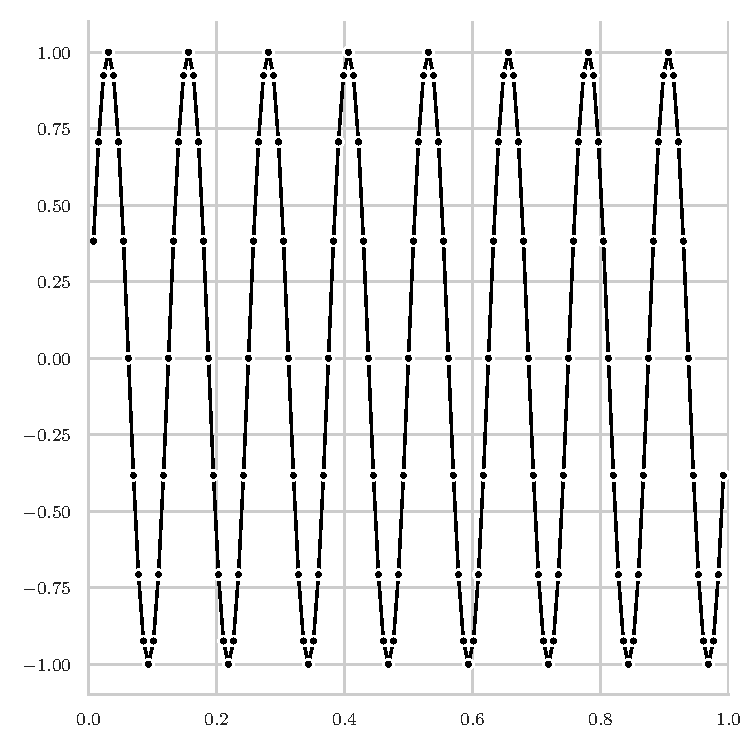
\includegraphics[width=\textwidth]{figures/error_plots//initial_error_16pi_level7.pdf}
	\end{subfigure}
	\hfill
	\begin{subfigure}[b]{0.32\textwidth}
		\centering
		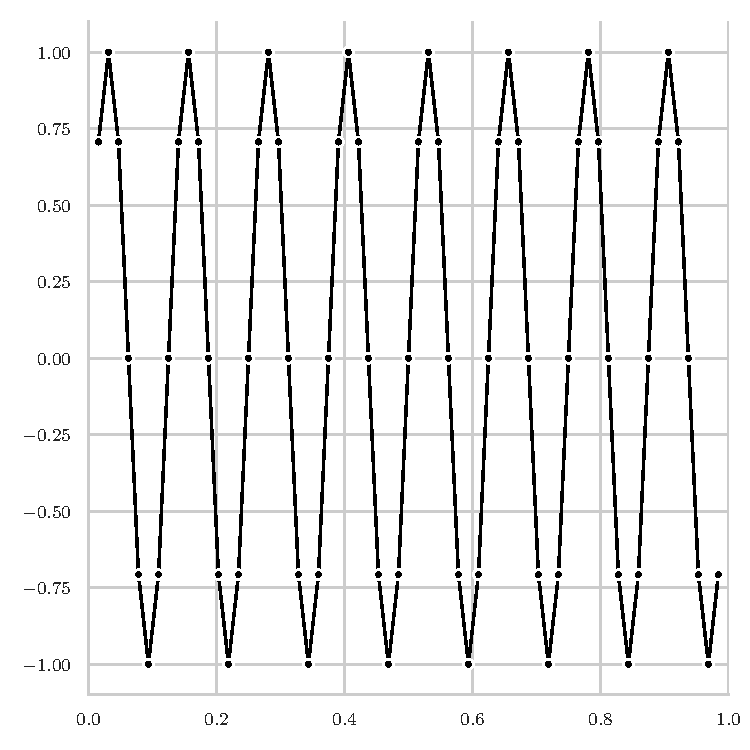
\includegraphics[width=\textwidth]{figures/error_plots//initial_error_16pi_level6.pdf}
	\end{subfigure}
	\hfill
	\begin{subfigure}[b]{0.32\textwidth}
		\centering
		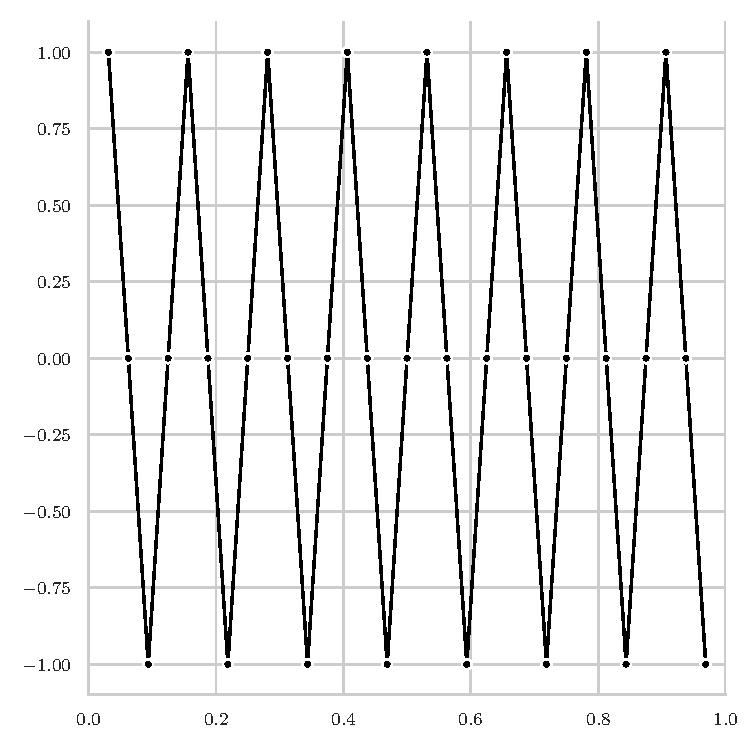
\includegraphics[width=\textwidth]{figures/error_plots//initial_error_16pi_level5.pdf}
	\end{subfigure}
		\begin{subfigure}[b]{0.32\textwidth}
		\centering
		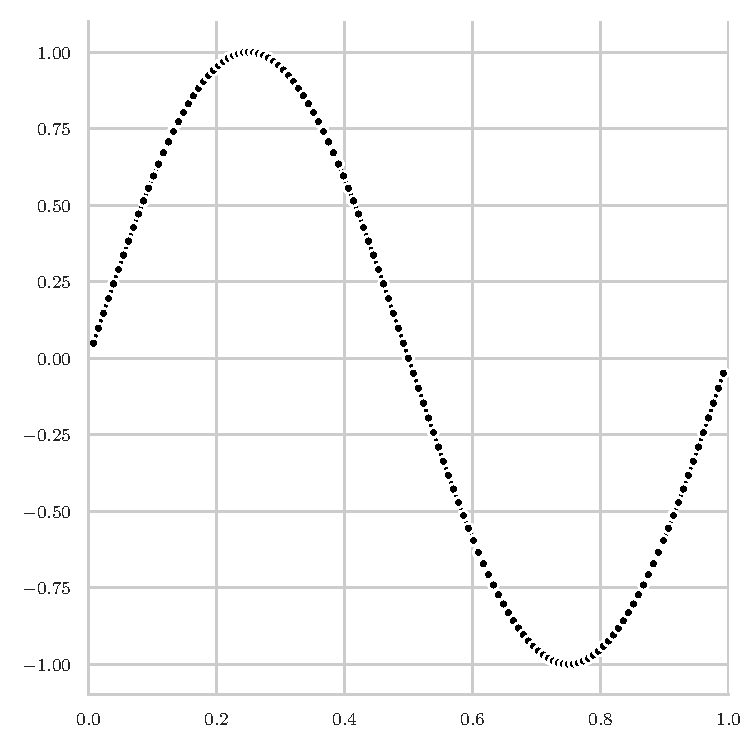
\includegraphics[width=\textwidth]{figures/error_plots//initial_error_2pi_level7.pdf}
		\caption{$h = 2^{-7}$}
	\end{subfigure}
	\hfill
	\begin{subfigure}[b]{0.32\textwidth}
		\centering
		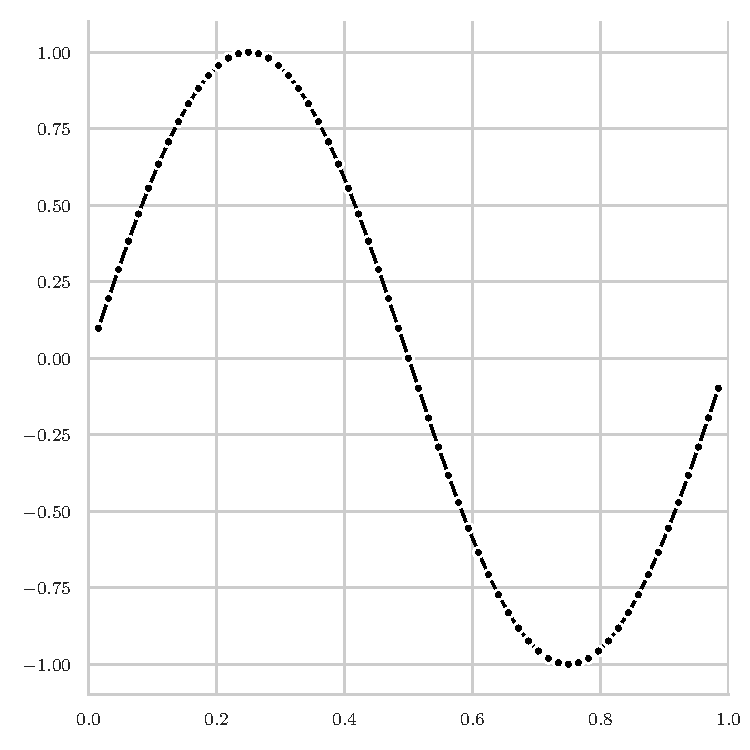
\includegraphics[width=\textwidth]{figures/error_plots//initial_error_2pi_level6.pdf}
		\caption{$h = 2^{-6}$}
	\end{subfigure}
	\hfill
	\begin{subfigure}[b]{0.32\textwidth}
		\centering
		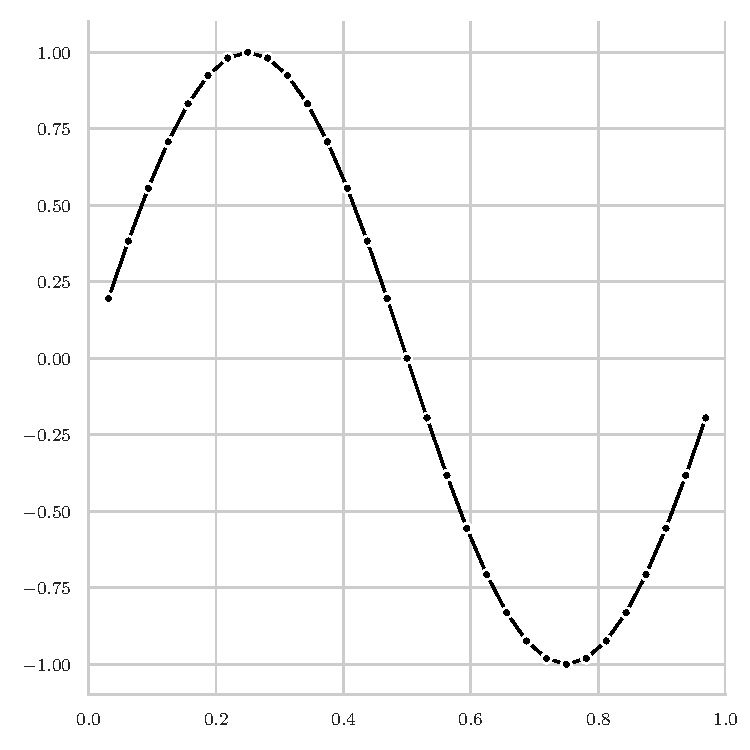
\includegraphics[width=\textwidth]{figures/error_plots//initial_error_2pi_level5.pdf}
		\caption{$h = 2^{-5}$}
	\end{subfigure}
	\caption{Oscillatory and smooth error components discretized on a hierarchy of grids with decreasing step size.}
	\label{fig:error-on-multiple-levels}
\end{figure}
Assuming that an error $\bm{e}_{2h}$ on the coarse grid consists exclusively of smooth components and, thus, $\bm{e}_{h} \approx I_{2h}^{h} \bm{e}_{2h}$, we can define a coarse-grid correction 
\begin{equation}
	\bm{x}^{(k+1)}_h = \bm{x}^{(k)}_h + I_{2h}^h \bm{e}_{2h}.
\end{equation} 
Now the question remains to be answered how we can compute an approximation for the error $\bm{e}_{2h}$ on the coarse grid.
As we have pointed out above, Equation~\eqref{eq:linear-system-error-equation} is equivalent to the original system.
We can, therefore, make use of our previously defined inter-grid transfer operators to define the error equation on a coarser grid with step size $2\bm{h}$
\begin{equation}
	\underbrace{I_{h}^{2h} A_h I_{2h}^h}_{A_{2h}} \bm{e}_{2h} = I_{h}^{2h} \left(\bm{b}_h - A_h \bm{x}^{(0)}_h\right).
	\label{eq:coarse-grid-error-equation}
\end{equation}
Note that we have again made use of the fact that in case $\bm{e}_{2h}$ is smooth, $\bm{e}_{h} \approx I_{2h}^{h} \bm{e}_{2h}$ is a reasonably accurate approximation.
Note that in Equation~\eqref{eq:coarse-grid-error-equation}, the coarse operator $A_{2h}$ is directly obtained from the original operator $A_{2h}$, which is called \emph{Galerkin coarsening}.
However, in cases where the operator $A_h$ can be directly discretized on a coarser grid with step size $2\bm{h}$, it is often also possible to use the resulting operator $A_{2h}$ instead.
By bringing all these components together, we can formulate the two-level-method shown in Algorithm~\ref{alg:two-grid-method}.
\begin{algorithm}
	\caption{Two-Grid Method}
	\label{alg:two-grid-method}
	\begin{algorithmic}
		\State{Smooth on $A_h \bm{x}_h = \bm{b}_h$ to obtain an approximation $\bm{x}_h$}
		\State{Compute the residual $\bm{r}_h = \bm{b}_h - A_h \bm{x}_h$}
		\State{\hskip1em Obtain $A_{2h}$ through Galerkin coarsening or rediscretization}
		\State{\hskip1em Restrict the residual $\bm{b}_{2h} = I_h^{2h} \bm{r}_h$}
		\State{\hskip1em Solve $A_{2h} \bm{x}_{2h} = \bm{b}_{2h}$ for $\bm{x}_{2h}$}
		\State{Perform the correction $\bm{x}_h = \bm{x}_h + I_{2h}^h \bm{x}_{2h}$}
		\State{Smooth again on $A_h \bm{x}_h = \bm{b}_h$ now using $\bm{x}_h$} as an initial guess
	\end{algorithmic}
\end{algorithm}
Note that while on the coarse grid, we are actually solving the error equation, it has been redefined as $A_{2h} \bm{x}_{2h} = \bm{b}_{2h}$.
Based on this notation, we could similarly define a two-level method starting from a grid with step size $2\bm{h}$.
However, to put this approach into practice, we need to choose an initial guess for the error equation on this level.
For this purpose, note that one step of smoothing applied to Equation~\eqref{eq:coarse-grid-error-equation} with an initial guess of zero corresponds to
\begin{equation}
	\bm{e}_{2h}^{(1)} = M_{2h}^{-1} I_{h}^{2h} \left(\bm{b}_h - A_h \bm{x}^{(0)}_h\right).
	\label{eq:initial-coarse-grid-relaxation}
\end{equation}
Since the error $\bm{e}_{2h}^{(k+1)}$ in step $k+1$ is defined as
\begin{equation*}
	\bm{e}_{2h}^{(k+1)} = \bm{x}_{2h}^{(k+1)} - \bm{x}_{2h}^{(k)},
\end{equation*}
and assuming that $\bm{x}_{h}^{(0)}$ is smooth, we can choose $\bm{x}_{2h}^{(0)} = I_{2h}^{h} \bm{x}_{h}^{(0)}$ and, hence, obtain the iteration
\begin{equation}
	\bm{x}_{2h}^{(1)} = I_{h}^{2h} \bm{x}_{h}^{(0)} + M_{2h}^{-1} ( I_{h}^{2h} \bm{b}_h - \underbrace{I_{h}^{2h} A_h I_{2h}^{h}}_{A_{2h}} I_{h}^{2h} \bm{x}_{h}^{(0)} ).
\end{equation}
Performing one smoothing step with an initial guess of zero on the coarse-grid error equation is, thus, similar to smoothing on the equation
\begin{equation}
	I_{h}^{2h} A_h I_{2h}^h \bm{x}_{2h} = I_{h}^{2h} \bm{b}_h,
\end{equation}
with an initial guess of $\bm{x}_{2h}^{(0)} = I_{h}^{2h} \bm{x}_{h}^{(0)}$.
Because smoothing aims to remove the remaining oscillatory components of the error that have been transferred from the fine grid, applying it in the form of Equation~\eqref{eq:initial-coarse-grid-relaxation} precisely serves this purpose.

\subsection{Restriction and Prolongation}
\label{subsec:restriction-and-prolongation}
%TODO fix stencil notation in this section
Before we can define an actual multigrid method, which recursively applies the techniques introduced in the last section to a hierarchy of discretizations consisting of more than two levels, we need to define suitable inter-grid operators, $I_{2h}^{h}$ and $I_{h}^{2h}$.
Here, the \emph{restriction} operator $I_{2h}^{h}$ is supposed to yield an accurate approximation of the current residual on a coarser grid, while the goal of the \emph{prolongation} operator $I_{h}^{2h}$ is to transfer the computed solution of the error equation back to a finer grid.
In both cases, we are, first and foremost, interested in preserving the low-frequency components, as all the others can already be quickly reduced by smoothing.
In general, the implementation of these operators depends on the chosen method of discretization. 
Since, as mentioned in Section~\ref{sec:discretization}, this work focuses on the discretizations of PDEs on regular grids, we do not consider inter-grid operators defined on other grid types, such as unstructured grids.
For a detailed treatment of these cases, the reader is referred to~\cite{trottenberg2000multigrid,ruge1987algebraic,stuben2001introduction}.
As a first step towards defining a suitable restriction operator, note that on a regular grid, the set of coarse-grid points is always contained in the set of fine-grid points.
Therefore, the easiest way to define such an operator is to simply carry over the values present at the respective points of the fine grid over to the coarse grid, which leads to the so-called \emph{injection} restriction operator.
While this approach might lead to a functioning multigrid method in case the residual is sufficiently smooth, it neglects the information contained within all fine grid points that do not coincide with one on the coarse grid.
In most cases, it is beneficial to incorporate this information into the coarse grid by computing a weighted average over all neighboring fine grid points.
This idea leads to the so-called \emph{full-weighting} and \emph{half-weighting} restriction operators.
Using our previously defined stencil notation, the one-dimensional full-weighting restriction operator is given by
\begin{equation}
	I_{h_x}^{2 h_x} = \frac{1}{4}\{((-1), 1), ((0), 2), ((1), 1)\}_{h_x}^{2h_x},
\end{equation} 
or equivalently using the matrix notation
\begin{equation}
	I_{h_x}^{2h_x} =  \frac{1}{4} \begin{bmatrix}
			1 & 2 & 1
		\end{bmatrix}_{h_x}^{2h_x}.
	\label{eq:full-weighting-restriction}
\end{equation} 
Since the application of this stencil yields a grid function of different dimensionality than the one to which it is applied, we additionally include the respective step sizes as a sub- and superscript.
If we treat Equation~\eqref{eq:full-weighting-restriction} as a row vector, we can define the two- and three-dimensional full-weighting restriction operator as a tensor product with the corresponding column vector, such that
\begin{equation}
	I^{2h_x, 2h_y}_{h_x, h_y} = \frac{1}{4} \begin{bmatrix}
		1 \\ 2 \\ 1
	\end{bmatrix}_{h_y}^{2h_y} \otimes \frac{1}{4} \begin{bmatrix}
		1 & 2 & 1
	\end{bmatrix}_{h_x}^{2h_x} =
\frac{1}{16} 
\begin{bmatrix}
	1 & 2 & 1 \\
	2 & 4 & 2 \\
	1 & 2 & 1
\end{bmatrix}^{2h_x, 2h_y}_{h_x, h_y}
\end{equation} 
\begin{equation}
\begin{split}
	& I^{2h_x, 2h_y, 2h_z}_{h_x, h_y, h_z} = \frac{1}{4} \begin{bmatrix}
		1 & 2 & 1
	\end{bmatrix}_{h_z}^{2h_z} \otimes 
	\frac{1}{16} 
	\begin{bmatrix}
		1 & 2 & 1 \\
		2 & 4 & 2 \\
		1 & 2 & 1
	\end{bmatrix}^{2h_x, 2h_y}_{h_x, h_y} \\
& = \frac{1}{64} \begin{bmatrix}
\begin{bmatrix}
	1 & 2 & 1 \\
	2 & 4 & 2 \\
	1 & 2 & 1
\end{bmatrix} &	\begin{bmatrix}
2 & 4 & 2 \\
4 & 8 & 4 \\
2 & 4 & 2
\end{bmatrix} &
\begin{bmatrix}
	1 & 2 & 1 \\
	2 & 4 & 2 \\
	1 & 2 & 1
\end{bmatrix}
\end{bmatrix}^{2h_x, 2h_y, 2h_z}_{h_x, h_y, h_z}
\end{split}
\end{equation}
A second restriction operator based on the idea of averaging neighboring fine grid points is the half-weighting restriction operator, whose two- and three-dimensional versions can be defined as
\begin{equation}
	I^{2h_x,2h_y}_{h_x, h_y} = \frac{1}{8}
	\begin{bmatrix}
		0 & 1 & 0 \\
		1 & 4 & 1 \\
		0 & 1 & 0
	\end{bmatrix}^{2h_x, 2h_y}_{h_x, h_y}
\end{equation} 
\begin{equation}
	I^{2h_x, 2h_y, 2h_z}_{h_x, h_y, h_z} = 
\frac{1}{12} \begin{bmatrix}
	\begin{bmatrix}
		0& 0 & 0 \\
		0 & 1 & 0 \\
		0& 0 & 0
	\end{bmatrix}
 &		\begin{bmatrix}
 	0 & 1 & 0 \\
 	1 & 6 & 1 \\
 	0 & 1 & 0
 \end{bmatrix} &
	\begin{bmatrix}
		0& 0 & 0 \\
		0 & 1 & 0 \\
		0& 0 & 0
	\end{bmatrix}
\end{bmatrix}^{2h_x, 2h_y, 2h_z}_{h_x, h_y, h_z}
\end{equation} 
% \begin{equation}
% \begin{split}
% 	& I^{2h_x, 2h_y, 2h_z}_{h_x, h_y, h_z} = 
% \frac{1}{4} \begin{bmatrix}
% 	1 & 2 & 1
% \end{bmatrix}_{h_z}^{2h_z}
% \otimes 
% \frac{1}{8}
% 	\begin{bmatrix}
% 	0 & 1 & 0 \\
% 	1 & 4 & 1 \\
% 	0 & 1 & 0 
% \end{bmatrix}^{2h_x,2h_y}_{h_x, h_y} \\
% & =
% \frac{1}{32} \begin{bmatrix}
% 	\begin{bmatrix}
% 		0& 1 & 0 \\
% 		1 & 4 & 1 \\
% 		0& 1 & 0
% 	\end{bmatrix}
%  &		\begin{bmatrix}
%  	0 & 2 & 0 \\
%  	2 & 6 & 2 \\
%  	0 & 2 & 0
%  \end{bmatrix} &
% 	\begin{bmatrix}
% 	0& 1 & 0 \\
% 	1 & 4 & 1 \\
% 	0& 1 & 0
% \end{bmatrix}
% \end{bmatrix}^{2h_x, 2h_y, 2h_z}_{h_x, h_y, h_z}
% \end{split}
% \end{equation} 
Note that in contrast to our original definition of the stencil application in Equation~\eqref{eq:stencil-application}, the restriction stencils presented here only have to be applied to each point on the fine grid that coincides with a coarse-grid point.
We can thus replace it with the following slightly adapted definition of stencil application
\begin{equation}
	\begin{split}
		& I_{h}^{2h} \cdot u_h(\bm{x}) = \sum_{k=1}^m b_k u_h({\bm x + \bm{a}_k} \circ \bm{h}) \quad 
		\text{with} \; \bm{x} \in G_{2h}, m \in \mathbb{N} \\ & (\bm{a}_k, b_k) \in I_{h}^{2h} \; \forall \, k \in \{ 1, 2, \dots, m \},
	\end{split}
	\label{eq:stencil-restriction-application}
\end{equation}
where $u_h(\bm{x})$ with $\bm{x} \in G_{2h} \supset G_h$ represents an arbitrary point on the fine grid for which there exists a unique coarse-grid point defined at the same spatial position within the computational domain.
Note that this is an immediate consequence of the fact that we have defined the set of coarse-grid points as a subset of the fine-grid points.

On the other hand, for prolongation, our goal is to define an operator that transfers an approximation of the error computed on a certain discretization level to a grid of higher resolution.
Therefore, we must be able to restore a larger number of grid points based on the given values on the coarse grid, which can be regarded as a distribution process.
The application of this operator to a given coarse-grid point $u_{2h}(\bm{x})$ with $\bm{x} \in G_{2h}$ can be defined as
\begin{equation}
	I_{2h}^{h} \cdot u_{2h}(\bm{x}) \rightarrow
	\begin{cases}
		& \forall \, (\bm{a}_k, b_k) \in I_{2h}^{h} \; \text{with} \; k \in \{ 1, 2, \dots, m \} \; \wedge \; \bm{x} \in G_{2h} : \\
		& u_{h}(\bm{x} + \bm{a}_k \circ \bm{h}) = u_{h}(\bm{x} + \bm{a}_k \circ \bm{h}) + b_k u_{2h}(\bm{x}), 
	\end{cases}
	\label{eq:stencil-prolongation application}
\end{equation}
where we assume that initially $\forall u_h(\bm{x}) \; \text{with} \; \bm{x} \in \mathcal G_h : u_h(\bm{x}) = 0$.
A common choice for one-dimensional prolongation is the linear interpolation operator~\cite{trottenberg2000multigrid}, which can be defined as
\begin{equation}
	I_{2h_x}^{h_x} =  \frac{1}{2} \begin{bmatrix}
		1 & 2 & 1
	\end{bmatrix}_{2h_x}^{h_x}.
	\label{eq:linear-interpolation}
\end{equation}
Similar to full-weighting restriction, we can derive two- and three-dimensional versions of this operator as tensor products of the form
\begin{equation}
	I_{2h_x, 2h_y}^{h_x, h_y} = \frac{1}{2} \begin{bmatrix}
		1 \\ 2 \\ 1
	\end{bmatrix}_{2h_y}^{h_y} \otimes \frac{1}{2} \begin{bmatrix}
		1 & 2 & 1
	\end{bmatrix}_{2h_x}^{h_x} =
	\frac{1}{4} 
	\begin{bmatrix}
		1 & 2 & 1 \\
		2 & 4 & 2 \\
		1 & 2 & 1
	\end{bmatrix}_{2h_x, 2h_y}^{h_x, h_y}
\end{equation}
\begin{equation}
	\begin{split}
		I_{2h_x, 2h_y, 2h_z}^{h_x, h_y, h_z} = & \frac{1}{2} \begin{bmatrix}
			1 & 2 & 1
		\end{bmatrix}_{2h_z}^{h_z} \otimes 
		\frac{1}{4} 
		\begin{bmatrix}
			1 & 2 & 1 \\
			2 & 4 & 2 \\
			1 & 2 & 1
		\end{bmatrix}_{2h_x,2h_y}^{h_x,h_y} \\
		= & \frac{1}{8} \begin{bmatrix}
			\begin{bmatrix}
				1 & 2 & 1 \\
				2 & 4 & 2 \\
				1 & 2 & 1
			\end{bmatrix}&	\begin{bmatrix}
				2 & 4 & 2 \\
				4 & 8 & 4 \\
				2 & 4 & 2
			\end{bmatrix} &
			\begin{bmatrix}
				1 & 2 & 1 \\
				2 & 4 & 2 \\
				1 & 2 & 1
			\end{bmatrix}
		\end{bmatrix}_{2h_x,2h_y,2h_z}^{h_x,h_y,h_z}
	\end{split}
\end{equation}
Finally, we want to emphasize that while the prolongation and restriction operators presented here represent a common choice for regular grids with uniform step sizes, for instance, the discretization of PDEs with varying coefficients often necessitates the use of more complex operators, such as~\cite{dendy1982black}.

\subsection{The Multigrid Cycle}\label{sec:multigrid-cycles}
By putting this all together, we can now implement a recursive version of Algorithm~\ref{alg:two-grid-method} that allows us to perform an arbitrary number of coarsening steps until the resulting system of linear equation is small enough to be solved directly.
The corresponding implementation of a \emph{multigrid cycle} in the form of the function \textsc{mg-cycle} is shown in Algorithm~\ref{alg:multigrid-cycle}.
\begin{algorithm}[h]
	\caption{Multigrid Cycle}
	\label{alg:multigrid-cycle}
	\begin{algorithmic}
		\Function{mg-cycle}{$k$, $\gamma$, $\bm{x}_h$, $A_h$, $\bm{b}_h$, $\nu_1$, $\nu_2$, $\omega$}
		\For{$i = 1, \dots, \nu_1$}
		\State{$\bm{x}_h = \bm{x}_h + \omega M_h^{-1} \left( \bm{b}_h - A_h \bm{x}_h \right)$ where $A_h = M_h + N_h$}
		\EndFor
		\State{$\bm{r}_h = \bm{b}_h - A_h \bm{x}_h$}
		\State{$\bm{b}_{2h} = I_h^{2h} \bm{r}_h$}
		\If{$k = 1$}
		\State{ Solve $A_{2h} \bm{x}_{2h} = \bm{b}_{2h}$ for $\bm{x}_{2h}$}
		\Else
		\State{$\bm{x}_{2h} = 0$}
		\For{$i = 1, \dots, \gamma$}
		\State{$\bm{x}_{2h} =  \textsc{mg-cycle}(\bm{x}_{2h}, A_{2h}, \bm{b}_{2h}, k-1, \gamma, \nu_1, \nu_2)$}
		\EndFor
		\EndIf
		\State{$\bm{x}_h = \bm{x}_h + I_{2h}^h \bm{x}_{2h}$}
		\For{$i = 1, \dots, \nu_2$}
		\State{$\bm{x}_h = \bm{x}_h + \omega M_h^{-1} \left( \bm{b}_h - A_h \bm{x}_h \right)$ where $A_h = M_h + N_h$}
		\EndFor
		\State \Return{$\bm{x}_h$}
		\EndFunction
	\end{algorithmic}
\end{algorithm}
Note that this function has a number of additional parameters compared to our original two-grid method.
First of all, $k$ defines the number of discretization levels and, thus, determines how many recursive coarsening steps need to be performed until the respective system of linear equations is solved directly.
Furthermore, since sometimes a single recursive application of this function is not sufficient to obtain a reasonably accurate approximation on the coarse grid, additional coarse-grid correction steps can be performed, as controlled by the parameter $\gamma$.
Finally, the parameters $\nu_1$ and $\nu_2$ specify the number of smoothing steps before and after the coarse-grid correction is performed, respectively.
Note that when applying multiple sweeps of smoothing or coarse-grid correction, the initial guess is replaced by the approximation obtained in the previous step.
While, in principle, the parameters of \textsc{mg-cycle} can be freely chosen, one usually classifies multigrid cycles according to the choice of $\gamma$, as each value yields a distinct computational pattern.
For instance, choosing $\gamma = 1$ means that only a single recursive descent is performed on each discretization level.
Figure~\ref{fig:three-grid-cycles} and~\ref{fig:four-grid-cycles} illustrate the algorithmic structure resulting from different values of $\gamma$ on a hierarchy of three and four grids, respectively.
Each white node corresponds to one or multiple steps of smoothing on the respective level, while a black node implies that the resulting error equation is solved directly.
%TODO fix these figures
\begin{figure}
	\captionsetup{justification=centering}
   \begin{subfigure}[t!]{0.075\textwidth}
		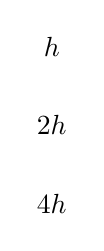
\begin{tikzpicture}
			\node   (h) at (-0.75, 4){$h$};
			\node   (2h) at (-0.75, 3){$2h$};
			\node   (4h) at (-0.75, 2){$4h$};
		\end{tikzpicture}
		\subcaption*{\phantom{$\gamma = 1$}}
	\end{subfigure}
	\begin{subfigure}[t!]{0.21\textwidth}
		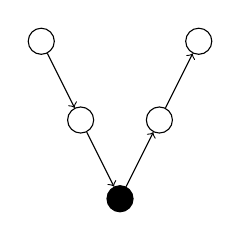
\begin{tikzpicture}
			\node	(a) at (0,4) [draw, circle,scale=1] {};
			\node	(b) at (0.5,3) [draw, circle,scale=1] {};
			\node	(c) at (1,2) [draw,circle,fill=black,scale=1] {};
			\node	(d) at (1.5,3) [draw, circle,scale=1] {};
			\node	(e) at (2,4) [draw, circle, scale=1] {};
			\draw 
			(a) edge[->] (b) 
			(b) edge[->] (c)
			(c) edge[->] (d)
			(d) edge[->] (e)   
			;
		\end{tikzpicture}
		\subcaption*{$\gamma = 1$}
	\end{subfigure}
	\begin{subfigure}[t!]{0.29\textwidth}
		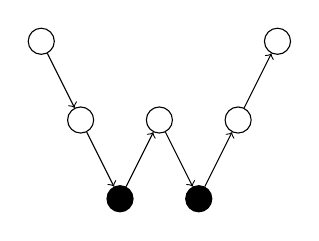
\begin{tikzpicture}
			\node	(a) at (0,4) [draw, circle,scale=1] {};
			\node	(b) at (0.5,3) [draw, circle,scale=1] {};
			\node	(c) at (1,2) [draw, circle,fill=black,scale=1] {};
			\node	(d) at (1.5,3) [draw, circle,scale=1] {};
			\node	(e) at (2,2) [draw, circle, fill=black, scale=1] {};
			\node	(f) at (2.5,3) [draw, circle, scale=1] {};
			\node	(g) at (3,4) [draw, circle, scale=1] {};
			
			\draw 
			(a) edge[->] (b) 
			(b) edge[->] (c)
			(c) edge[->] (d)
			(d) edge[->] (e)   
			(e) edge[->] (f)
			(f) edge[->] (g)
			;
		\end{tikzpicture}
		\subcaption*{$\gamma = 2$}
	\end{subfigure}
	\begin{subfigure}[t!]{0.35\textwidth}
		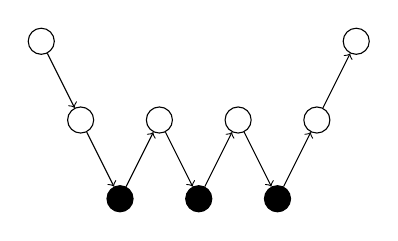
\begin{tikzpicture}
			\node	(a) at (0,4) [draw, circle,scale=1] {};
			\node	(b) at (0.5,3) [draw, circle,scale=1] {};
			\node	(c) at (1,2) [draw, circle,fill=black,scale=1] {};
			\node	(d) at (1.5,3) [draw, circle,scale=1] {};
			\node	(e) at (2,2) [draw, circle, fill=black, scale=1] {};
			\node	(f) at (2.5,3) [draw, circle, scale=1] {};
			\node	(g) at (3,2) [draw, circle, fill=black,scale=1] {};
			\node	(h) at (3.5,3) [draw, circle, scale=1] {};	
			\node	(i) at (4,4) [draw, circle, scale=1] {};	
			\draw 
			(a) edge[->] (b) 
			(b) edge[->] (c)
			(c) edge[->] (d)
			(d) edge[->] (e)   
			(e) edge[->] (f)
			(f) edge[->] (g)
			(g) edge[->] (h)
			(h) edge[->] (i)
			;
		\end{tikzpicture}
		\subcaption*{$\gamma = 3$}
	\end{subfigure}
	\caption{Three-grid cycles ($k = 3$).}
	\label{fig:three-grid-cycles}
\end{figure}
\begin{figure}
	\captionsetup{justification=centering}
	\begin{subfigure}[t!]{0.075\textwidth}
		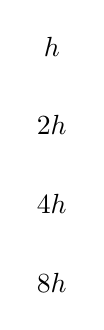
\begin{tikzpicture}
			\node   (h) at (-0.75, 4){$h$};
			\node   (2h) at (-0.75, 3){$2h$};
			\node   (4h) at (-0.75, 2){$4h$};
			\node   (8h) at (-0.75, 1){$8h$};
		\end{tikzpicture}
		\subcaption*{\phantom{$\gamma = 1$}}
	\end{subfigure}
	\begin{subfigure}[t!]{0.295\textwidth}
		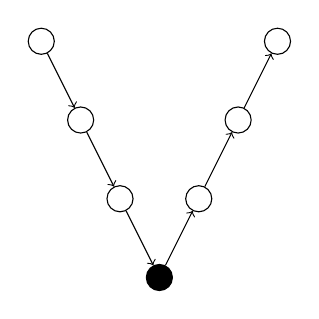
\begin{tikzpicture}
			\node	(a) at (0,4) [draw, circle,scale=1] {};
			\node	(b) at (0.5,3) [draw, circle,scale=1] {};
			\node	(c) at (1,2) [draw, circle,scale=1] {};
			\node	(d) at (1.5,1) [draw, circle,fill=black, scale=1] {};
			\node	(e) at (2,2) [draw, circle, scale=1] {};
			\node	(f) at (2.5,3) [draw, circle,scale=1] {};
			\node	(g) at (3,4) [draw, circle,scale=1] {};
			\draw 
			(a) edge[->] (b) 
			(b) edge[->] (c)
			(c) edge[->] (d)
			(d) edge[->] (e)   
			(e) edge[->] (f)
			(f) edge[->] (g)
			
			;
		\end{tikzpicture}
		\subcaption*{$\gamma = 1$}
	\end{subfigure}
	\begin{subfigure}[t!]{0.59\textwidth}
		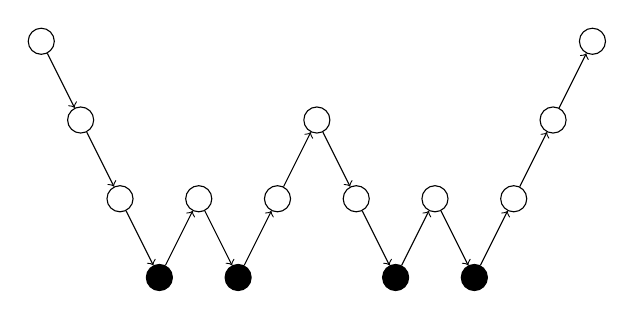
\begin{tikzpicture}
			\node	(a) at (0,4) [draw, circle,scale=1] {};
			\node	(b) at (0.5,3) [draw, circle,scale=1] {};
			\node	(c) at (1,2) [draw, circle,scale=1] {};
			\node	(d) at (1.5,1) [draw, circle,fill=black, scale=1] {};
			\node	(e) at (2,2) [draw, circle, scale=1] {};
			\node	(f) at (2.5,1) [draw, circle,fill=black,scale=1] {};
			\node	(g) at (3,2) [draw, circle,scale=1] {};
			\node	(h) at (3.5,3) [draw, circle,scale=1] {};
			\node	(i) at (4,2) [draw, circle,scale=1] {};
			\node	(j) at (4.5,1) [draw, circle,fill=black, scale=1] {};
			\node	(k) at (5,2) [draw, circle, scale=1] {};
			\node	(l) at (5.5,1) [draw, circle,fill=black,scale=1] {};
			\node	(m) at (6,2) [draw, circle,scale=1] {};
			\node	(n) at (6.5,3) [draw, circle, scale=1] {};
			\node	(o) at (7,4) [draw, circle, scale=1] {};
			
			\draw 
			(a) edge[->] (b) 
			(b) edge[->] (c)
			(c) edge[->] (d)
			(d) edge[->] (e)   
			(e) edge[->] (f)
			(f) edge[->] (g)
			(g) edge[->] (h)
			(h) edge[->] (i)
			(i) edge[->] (j)
			(j) edge[->] (k)
			(k) edge[->] (l)
			(l) edge[->] (m)
			(m) edge[->] (n)
			(n) edge[->] (o)
			;
		\end{tikzpicture}
		\subcaption*{$\gamma = 2$}
	\end{subfigure}
	\caption{Four-grid cycles ($k = 4$).}
	\label{fig:four-grid-cycles}
\end{figure}
Since, as it can be seen in Figure~\ref{fig:three-grid-cycles}, the choice of $\gamma = 1$ results in a V-shaped computational pattern, the corresponding multigrid method is usually called a V-cycle.
Similarly, the computational pattern of a method with $\gamma = 2$ on a three-grid hierarchy looks like the letter W, and hence the resulting method is called a W-cycle.
As it can be seen in Figure~\ref{fig:four-grid-cycles}, the amount of computational work within a W-cycle drastically increases with the number of coarsening steps.
While applying a V-cycle always results in significantly fewer computations, in many cases, a single coarse-grid correction step is not sufficient to reduce the low-frequency components of the initial error on the finest grid~\cite{trottenberg2000multigrid}.
Due to the resulting drastic increase in the number of computations, values of $\gamma$ larger than two are usually impractical for multigrid methods.
While Algorithm~\ref{alg:multigrid-cycle} enables the realization of different multigrid methods based on choosing different values for the parameters $k$, $\gamma$, $\nu_1$, $\nu_2$ and $\omega$, the structural composition of the resulting methods is limited.
For instance, in Algorithm~\ref{alg:multigrid-cycle}, it is assumed that the same value of $\gamma$ is chosen on each level, which restricts the set of possible multigrid cycles to those portrayed in Figure~\ref{fig:three-grid-cycles} and~\ref{fig:four-grid-cycles}.
One way to overcome this limitation is to combine different cycle types in a single method.
For instance, combining W- and V-cycles on each level results in a so-called F-cycle, whose algorithmic structure is illustrated in Figure~\ref{fig:f-cycle}.
\begin{figure}
	\begin{subfigure}[t]{0.4\textwidth}
		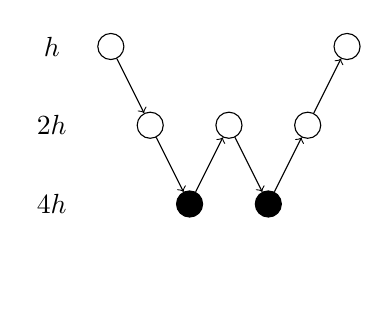
\begin{tikzpicture}
			\node   (h) at (-0.75, 4){$h$};
			\node   (2h) at (-0.75, 3){$2h$};
			\node   (4h) at (-0.75, 2){$4h$};
			\node   (8h) at (-0.75, 1){\phantom{$8h$}};
			\node	(a) at (0,4) [draw, circle,scale=1] {};
			\node	(b) at (0.5,3) [draw, circle,scale=1] {};
			\node	(c) at (1,2) [draw, circle,fill=black,scale=1] {};
			\node	(d) at (1.5,3) [draw, circle,scale=1] {};
			\node	(e) at (2,2) [draw, circle, fill=black, scale=1] {};
			\node	(f) at (2.5,3) [draw, circle, scale=1] {};
			\node	(g) at (3,4) [draw, circle, scale=1] {};
			
			\draw 
			(a) edge[->] (b) 
			(b) edge[->] (c)
			(c) edge[->] (d)
			(d) edge[->] (e)   
			(e) edge[->] (f)
			(f) edge[->] (g)
			;
		\end{tikzpicture}
  		\subcaption*{}
	\end{subfigure}
	\begin{subfigure}[t]{0.59\textwidth}
		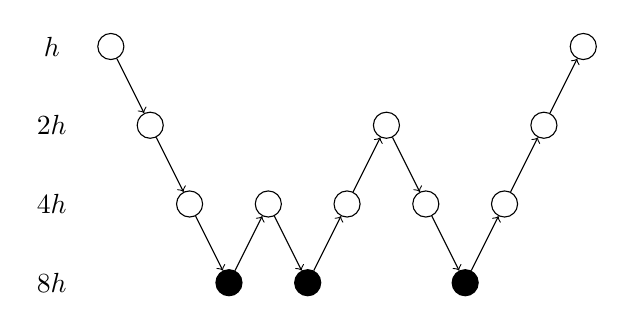
\begin{tikzpicture}
				\node   (h) at (-0.75, 4){$h$};
				\node   (2h) at (-0.75, 3){$2h$};
				\node   (4h) at (-0.75, 2){$4h$};
				\node   (8h) at (-0.75, 1){$8h$};
			\node	(a) at (0,4) [draw, circle,scale=1] {};
			\node	(b) at (0.5,3) [draw, circle,scale=1] {};
			\node	(c) at (1,2) [draw, circle,scale=1] {};
			\node	(d) at (1.5,1) [draw, circle,fill=black, scale=1] {};
			\node	(e) at (2,2) [draw, circle, scale=1] {};
			\node	(f) at (2.5,1) [draw, circle,fill=black,scale=1] {};
			\node	(g) at (3,2) [draw, circle,scale=1] {};
			\node	(h) at (3.5,3) [draw, circle,scale=1] {};
			\node	(i) at (4,2) [draw, circle,scale=1] {};
			\node	(j) at (4.5,1) [draw, circle,fill=black, scale=1] {};
			\node	(k) at (5,2) [draw, circle, scale=1] {};
			\node	(l) at (5.5,3) [draw, circle,scale=1] {};
			\node	(m) at (6,4) [draw, circle,scale=1] {};
			
			\draw 
			(a) edge[->] (b) 
			(b) edge[->] (c)
			(c) edge[->] (d)
			(d) edge[->] (e)   
			(e) edge[->] (f)
			(f) edge[->] (g)
			(g) edge[->] (h)
			(h) edge[->] (i)
			(i) edge[->] (j)
			(j) edge[->] (k)
			(k) edge[->] (l)
			(l) edge[->] (m)
			;
		\end{tikzpicture}
    		\subcaption*{}
	\end{subfigure}
	\caption{Computational pattern of the F-cycle with a different number of coarsening steps.}
	\label{fig:f-cycle}
\end{figure}
Except for $k = 3$, in which case the F-cycle and W-cycle are equivalent, this method represents a compromise between a pure V-cycle and W-cycle.
While the composition of a multigrid method from different cycle types represents an additional degree of freedom, the individual cycles are still derived from the rules of Algorithm~\ref{alg:multigrid-cycle} and are, thus, fully described by the aforementioned parameters.
Since, according to the classical formulation of a multigrid method as in~\cite{brandt1977multi,hackbusch2013multi,trottenberg2000multigrid,briggs2000multigrid}, these parameters are considered global, adapting one of their values uniformly changes the method's behavior on each level. 
While for many applications, this approach has demonstrated to yield efficient multigrid methods~\cite{trottenberg2000multigrid}, there are still cases where multigrid could not yet achieve its full potential~\cite{ernst2012difficult,benzi2005numerical}.
Even though, to date, there exists a rich amount of research on the optimization of multigrid cycles based on a fixed set of global parameters, the variation of its components on an individual level has not been considered yet.
Such an approach would grant the flexibility to generate multigrid cycles that consist of varying restriction and coarse-grid correction steps, each with a different combination of smoothers and relaxation factors.
In this work, we aim to realize this vision by expressing each multigrid cycle as a finite sequence of instructions whose order is restricted by the rules of linear algebra and multigrid theory.
To specify these rules in a mathematically formal way, we make use of programming language theory, such that the design of an efficient multigrid method can be treated as a program synthesis task.
In the next section, we, therefore, provide a brief overview of programming language theory and introduce the concept of formal languages and grammars.
We then leverage this formalism together with the theoretical background presented in this chapter to derive a grammar-based representation of multigrid cycles that enables us to automate the design of these methods using evolutionary program synthesis techniques.